\begin{problem}[1]
  Evaluate the following double integrals over the given regions.
  \begin{enumerate}
    \item $\displaystyle \iint_R ye^{xy} \,\dA$ where $R = [0, 2] \times [0,
      4]$.

    \item $\displaystyle \iint_D y\sqrt{x^2 - y^2} \,\dA$ where $D$ is the
      triangle with vertices $(0, 0)$, $(2, 0)$, and $(2, 2)$.

    \item $\displaystyle \iint_D 2xy^3 \,\dA$ where $D$ is the region bounded by $y = x$, $y = \frac{1}{x}$, and $y = 2$.
  \end{enumerate}
\end{problem}

\begin{proof}[Solution to (i)]
  Expanding the double integral into an iterated integral and evaluating gives
  us
  \begin{align*}
    \iint_R ye^{xy} \,\dA &= \int_0^4 \int_0^2 ye^{xy} \,\dx \,\dy \\
                          &= \int_0^4 \left[e^{xy}\right]_0^2 \,\dy \\
                          &= \int_0^4 e^{2y} - 1 \,\dy \\
                          &= \left[\frac{e^{2y}}{2} - y\right]_0^4 \\
                          &= \frac{1}{2}(e^8 - 9)
  .\qedhere\end{align*}
\end{proof}

\begin{proof}[Solution to (ii)]
  Graphing the bounds gives us
  \begin{center}
    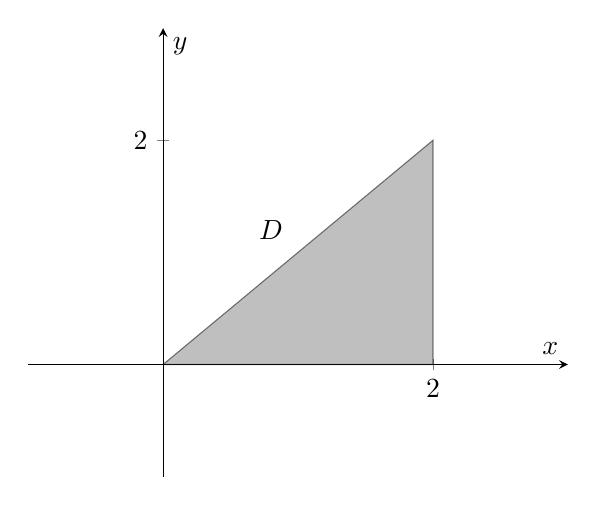
\begin{tikzpicture}
      \begin{axis}[
        axis lines = center,
        xlabel = $x$,
        ylabel = $y$,
        xmin = -1, xmax = 3,
        ymin = -1, ymax = 3,
        xtick = {0, 2},
        ytick = {0, 2},
        xticklabels = {$0$, $2$},
        yticklabels = {$0$, $2$},
      ]
        \addplot[fill=gray, opacity=0.5] coordinates {
          (0, 0) (2, 0) (2, 2) (0, 0)
        };
        \node at (axis cs: 0.8, 1.2) {$D$};
      \end{axis}
    \end{tikzpicture}
  \end{center}
  Therefore, we are given the $x$ bounds to be $0$ to $2$. The $y$ bounds are
  from $0$ to $x$. Expanding the double integral into an iterated integral gives
  us
  \[%
    \iint_D y\sqrt{x^2 - y^2} \,\dA = \int_0^2 \int_0^x y\sqrt{x^2 - y^2} \,\dy \,\dx
  .\]%
  Using a $u$-substitution of $u = y^2$, we have $\du = 2y\,\dy$. The bounds go
  from $0 \mapsto 0$ and $x \mapsto x^2$. This simplifies the integral to
  \begin{align*}
    \int_0^2 \int_0^x y\sqrt{x^2 - y^2} \,\dy \,\dx &= \int_0^2 \int_0^{x^2} \frac{1}{2} \sqrt{x^2 - u} \,\du \,\dx \\
                                                    &= \frac{1}{2} \int_0^2 \left.-\frac{(x^2 - u)^{\sfrac{3}{2}}}{\sfrac{3}{2}}\right\rvert_0^{x^2} \,\dx \\
                                                    &= \frac{1}{2} \int_0^2 \frac{2}{3}x^3 \,\dx = \frac{4}{3}
  .\qedhere\end{align*}
\end{proof}

\begin{proof}[Solution to (iii)]
  Graphing the bounds gives us
  \begin{center}
    \begin{tikzpicture}
      \begin{axis}[
        axis lines = center,
        xlabel = $x$,
        ylabel = $y$,
        xmin = 0.4, xmax = 2.4,
        ymin = 0.6, ymax = 2.4,
        ]
        \addplot[domain=1:2] {x} node[midway, right] {$y = x$};
        \addplot[domain=0.5:1] {1/x} node[midway, right] {$y = \frac{1}{x}$};
        \addplot[domain=0.5:2] {2} node[midway, below] {$y = 2$};
      \end{axis}
    \end{tikzpicture}
  \end{center}
  Therefore, we'll use a $y$-bounds are $1$ to $2$ and the $x$-bounds are from
  $y$ to $\frac{y}{y}$. Expanding the double integral into an iterated integral
  and evaluating gives us
  \begin{align*}
    \iint_D 2xy^3 \,\dA &= \int_1^2 \int_y^{\sfrac{1}{y}} 2xy^3 \,\dx \,\dy \\
                        &= \int_1^2 \left(\frac{1}{y^2} - y^2\right) y^3 \,\dy \\
                        &= \int_1^2 y - y^5 \,\dy \\
                        &= \int_1^2 y \,\dy - \int_1^2 y^5 \,\dy \\
                        &= -9
  .\qedhere\end{align*}
\end{proof}

\begin{problem}[2]
  By changing the order of integration, evaluate the integral
  \[%
    \int_0^2 \int_{x^2}^4 \sqrt{x} \sin(y) \,\dy \,\dx
  .\]%
\end{problem}

\begin{proof}[Solution]
  Solving the equation $y = x^2$ gives us $x = \pm \sqrt{y}$. So, we get the new
  bounds of $4 \le y \le 0$ and $0 \le x \le \sqrt{y}$. Expanding the double
  integral into an iterated integral and evaluating gives us
  \begin{align*}
    \int_0^2 \int_{x^2}^4 \sqrt{x} \sin(y) \,\dy \,\dx &= \int_0^4 \int_0^{\sqrt{y}} \sqrt{x} \sin(y) \,\dx \,\dy \\
                                                       &= \int_0^4 \sin(y) \int_0^{\sqrt{y}} \sqrt{x} \,\dx \,\dy \\
                                                       &= \int_0^4 \sin(y) \left[\frac{2}{3}x^{\sfrac{3}{2}}\right]_0^{\sqrt{y}} \,\dy \\
                                                       &= \frac{2}{3}\int_0^4 \sin(y) y^{\sfrac{3}{4}} \,\dy
  .\end{align*}
\end{proof}

\begin{problem}[3]
  Use a double integral to find the volume of the following solids.
  \begin{enumerate}
    \item The solid that is bounded by the coordinate planes and the plane $2x +
      3y + z = 6$.

      Note: This solid is a tetrahedron. It can be easily drawn by using the
      lines of intersection between the slant plane and the coordinate planes.

    \item The solid enclosed by the parabolic cylinder $y = 2 - x^2$ and the
      planes $z = 1 - y$, $y = x$, and $z = 0$

      Note : Surfaces that do not depend on $z$ are vertical surfaces.
  \end{enumerate}
\end{problem}

\begin{proof}[Solution to (i)]
\end{proof}

\begin{proof}[Solution to (ii)]
\end{proof}
